\input{header.tex}

\title{Whitehead Product}
\author{Yannis B\"{a}hni}
\address[Yannis B\"{a}hni]{University of Zurich, R\"{a}mistrasse 71, 8006 Zurich}
\email[Yannis B\"{a}hni]{\href{mailto:yannis.baehni@uzh.ch}{\nolinkurl{yannis.baehni@uzh.ch}}}

\begin{document}

\begin{abstract}
	Aim of this paper is to give a short overview of the definition and the basic properties of the non-generalized \emph{Whitehead product}.
\end{abstract}

\maketitle

\tableofcontents

\section{Definition of the Whitehead Product}
Notice, that for any $(X,x_0),(Y,y_0) \in \mathsf{Top}_*$, their coproduct is given by
\begin{equation*}
	X \coprod Y = (X \times \cbr[0]{y_0}) \cup (\cbr[0]{x_0} \times Y) \subseteq X \times Y,
\end{equation*}
\noindent with basepoint $(x_0,y_0)$. 

\begin{lemma}
	\label{lem:attaching_cell_wedge_sum_spheres}
	Let $n,m \in \omega$, $n,m \geq 1$. The space $\mathbb{S}^n \times \mathbb{S}^m$ can be obtained from $\mathbb{S}^n \vee \mathbb{S}^m$ by attaching an $n + m$-cell.
\end{lemma}

\begin{proof}
	Observe, that $\mathbb{D}^{n + m} \cong \mathbb{D}^n \times \mathbb{D}^m$ and hence
	\begin{equation*}
		\mathbb{S}^{n + m - 1} = \partial \mathbb{D}^{n + m} \cong (\partial \mathbb{D}^n \times \mathbb{D}^m) \cup (\mathbb{D}^n \times \partial \mathbb{D}^m) = (\mathbb{S}^{n - 1} \times \mathbb{D}^m) \cup (\mathbb{D}^n \times \mathbb{S}^{m - 1}).
	\end{equation*}
	Let 
	\begin{equation*}
		f_1 : \mathbb{S}^{n - 1} \times \mathbb{D}^m \to (\mathbb{S}^{n - 1} \times \mathbb{D}^m) / (\mathbb{S}^{n - 1} \times \mathbb{S}^{m - 1}) \cong \ast \times \mathbb{S}^m
	\end{equation*}
	\noindent and
	\begin{equation*}
		f_2 : \mathbb{D}^n \times \mathbb{S}^{m - 1} \to (\mathbb{D}^n \times \mathbb{S}^{m - 1}) / (\mathbb{S}^{n - 1} \times \mathbb{S}^{m - 1}) \cong \mathbb{S}^n \times \ast
	\end{equation*}
	\noindent be the quotient maps. An application of the gluing lemma thus yields a map
	\begin{equation*}
		f : \mathbb{S}^{n + m - 1} \to \mathbb{S}^n \vee \mathbb{S}^m.
	\end{equation*}
	Moreover, define 
	\begin{equation*}
		q : \mathbb{D}^n \times \mathbb{D}^m \to \mathbb{D}^n/\mathbb{S}^{n - 1} \times \mathbb{D}^m/\mathbb{S}^{m - 1} \cong \mathbb{S}^n \times \mathbb{S}^m	
	\end{equation*}
	\noindent to be the product of quotient maps. Thus we get a commutative diagram
	\begin{equation*}
		\begin{tikzcd}
			\mathbb{S}^{n + m - 1} \arrow[r,"f"]\arrow[d,hook] & \mathbb{S}^n \vee \mathbb{S}^m \arrow[d,hook]\\
			\mathbb{D}^{n + m} \arrow[r,"q"'] & \mathbb{S}^n \times \mathbb{S}^m
		\end{tikzcd}
	\end{equation*}
	Suppose $(X,g,h)$ is another cocone for the pushout diagram:
	\begin{equation*}
		\begin{tikzcd}
			\mathbb{S}^{n + m - 1} \arrow[r,"f"]\arrow[d,hook] & \mathbb{S}^n \vee \mathbb{S}^m \arrow[d,hook]\arrow[ddr,bend left,"h"]\\
			\mathbb{D}^{n + m} \arrow[r,"q"']\arrow[drr,bend right,"g"'] & \mathbb{S}^n \times \mathbb{S}^m\\
			& & X.
		\end{tikzcd}
	\end{equation*}
	By \cite[186]{munkres:topology:2000}, $q$ is a quotient map. Moreover, for $(x,y) \in \mathbb{S}^{n - 1} \times \mathbb{S}^{m - 1}$, we have that
	\begin{equation*}
		g(x,y) = (h \circ f)(x,y) = h(\ast,\ast).
	\end{equation*}
	Thus $g$ passes to the quotient by \cite[72]{lee:topological_manifolds:2011} to yield a unique map
	\begin{equation*}
		\wtilde{g} : \mathbb{S}^n \times \mathbb{S}^m \to X,
	\end{equation*}
	\noindent such that $g = \wtilde{g} \circ q$. Finally, it is easy to check that
	\begin{equation*}
		\begin{tikzcd}
			\mathbb{S}^{n + m - 1} \arrow[r,"f"]\arrow[d,hook] & \mathbb{S}^n \vee \mathbb{S}^m \arrow[d,hook]\arrow[ddr,bend left,"h"]\\
			\mathbb{D}^{n + m} \arrow[r,"q"']\arrow[drr,bend right,"g"'] & \mathbb{S}^n \times \mathbb{S}^m\arrow[dr,"\wtilde{g}"]\\
			& & X.
		\end{tikzcd}
	\end{equation*}
	\noindent commutes.
\end{proof}

For $n,m \in \omega$, $n,m \geq 1$, consider the map $f$ from lemma \ref{lem:attaching_cell_wedge_sum_spheres}. Let $(X,p) \in \mathsf{Top}_*$. If $[\alpha] \in \pi_n(X,p)$ and $[\beta] \in \pi_m(X,p)$, we get two pointed maps
\begin{equation*}
	\alpha : \mathbb{S}^n \to X \qquad \text{and} \qquad \beta : \mathbb{S}^m \to X.
\end{equation*}
Forming their wedge $\alpha \vee \beta : \mathbb{S}^n \vee \mathbb{S}^m \to X$, defined by
\begin{align*}
	(\alpha \vee \beta) (x,y) := \ccases{
		\alpha(x) & y = \ast,\\
		\beta(y) & x = \ast,
	}
\end{align*}
\noindent and precomposing with $f$, yields a pointed map
\begin{equation*}
	(\alpha \vee \beta) \circ f : \mathbb{S}^{n + m - 1} \to X.
\end{equation*}
Explicitely, if we consider
\begin{equation*}
	\alpha : (\mathbb{D}^n,\mathbb{S}^{n - 1}) \to (X,p) \qquad \text{and} \qquad \beta : (\mathbb{D}^m,\mathbb{S}^{m - 1}) \to (X,p),
\end{equation*}
\noindent we get that
\begin{align*}
	\del[1]{(\alpha \vee \beta) \circ f}(x,y) = \ccases{
		\alpha(x) & x \in \mathbb{D}^n, y \in \mathbb{S}^{m - 1},\\
		\beta(y) & x \in \mathbb{S}^{n - 1}, y \in \mathbb{D}^m.
	}
\end{align*}
Hence if $F : \alpha \simeq_{\mathbb{S}^{n - 1}} \alpha'$ and $F' : \beta \simeq_{\mathbb{S}^{m - 1}} \beta'$, we get that 
\begin{equation*}
	H : \del[0]{(\alpha \vee \beta) \circ f} \simeq_\ast \del[0]{(\alpha' \vee \beta') \circ f},
\end{equation*}
\noindent where $H : \mathbb{S}^{n + m - 1} \times I \to X$ is defined by
\begin{align*}
	H(x,y,t) := \ccases{
		F(x,t) & x \in \mathbb{D}^n, y \in \mathbb{S}^{m - 1},\\
		F'(y,t) & x \in \mathbb{S}^{n - 1}, y \in \mathbb{D}^m.
	}
\end{align*}
Thus we get a well defined map $[-,-] : \pi_n(X) \times \pi_m(X) \to \pi_{n + m - 1}(X)$, defined by
\begin{equation*}
	[\alpha,\beta] := [(\alpha \vee \beta) \circ f].
\end{equation*}

\begin{definition}[Whitehead Product]
	Let $n,m \in \omega$, $n,m \geq 1$, and $(X,p) \in \mathsf{Top}_\ast$. The product
	\begin{equation*}
		[-,-] : \pi_n(X,p) \times \pi_m(X,p) \to \pi_{n + m - 1}(X,p)
	\end{equation*}
	\noindent defined by
	\begin{equation*}
		[\alpha,\beta] := [(\alpha \vee \beta) \circ f], 
	\end{equation*}
	\noindent is called the \bld{Whitehead product} and $[-,-]$ is called the \bld{Whitehead bracket}.
\end{definition}

\section{The Whitehead Product and the Conjugation Action}
In this section, we want to have a closer look at $[-,-] : \pi_1(X) \times \pi_n(X) \to \pi_n(X)$. From figure \ref{fig:n=1} we immediately deduce that
\begin{equation*}
	[\alpha,\beta] = [\alpha\beta\alpha^{-1}\beta^{-1}].
\end{equation*}
Thus $[\alpha,\beta]$ coincides with the notation of a commutator.\\
Let $n > 1$. Then it follows from figure \ref{fig:n>1}, that
\begin{equation*}
	[\alpha,\beta] = [\alpha \cdot \beta] - [\beta],
\end{equation*}
\noindent where $\alpha \cdot \beta$ denotes the \emph{conjugation action}, i.e. the action of $\pi_1(X)$ on $\pi_n(X)$.

\begin{figure}[h!tb]
	\begin{subfigure}[b]{0.5\textwidth}
		\centering
		\begin{tikzpicture}[scale = 6]
			\draw [thick] (0,0) -- (1,0);
			\draw [thick] (0,0) -- (0,1);
			\draw [thick] (1,0) -- (1,1);
			\draw [thick] (0,1) -- (1,1);
			\draw [thick,->] (0,0) -- (.5,0);
			\draw [thick,->] (1,0) -- (1,.5);
			\draw [thick,->] (0,1) -- (.5,1);
			\draw [thick,->] (0,0) -- (0,.5);
			\draw (.5,0) node[below] {$\alpha$};
			\draw (1,.5) node[right] {$\beta$};
			\draw (.5,1) node[above] {$\alpha$};
			\draw (0,.5) node[left] {$\beta$};
		\end{tikzpicture}
		\caption{$n = 1$.}
    	\label{fig:n=1}
	\end{subfigure}
	~
	\begin{subfigure}[b]{0.5\textwidth}
		\centering
		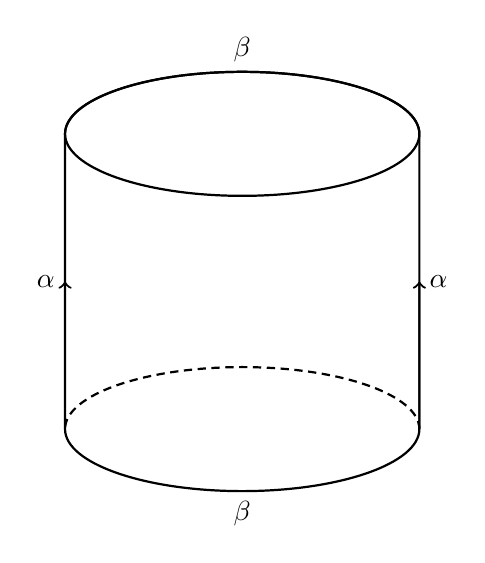
\begin{tikzpicture}[scale = 3]
			\draw [thick]
  				(180:7.5mm) coordinate (A)
				-- ++(0,-12.5mm) coordinate [midway] (E) coordinate (B) node [midway,left] {$\alpha$}
				arc (180:360:7.5mm and 2.625mm) coordinate (D) node [midway,below] {$\beta$}
				-- (A -| D) coordinate [midway] (F) coordinate (C) node [midway,right] {$\alpha$} arc (0:180:7.5mm and 2.625mm) node [midway,above] {$\beta$};
  			\draw [thick]
  				(0,0) coordinate (T) circle (7.5mm and 2.625mm);
  			\draw [thick,densely dashed] (D) arc (0:180:7.5mm and 2.625mm);
			\draw [thick,->] (B) -- (E);
			\draw [thick,->] (D) -- (F);
			\path [] (A) -- (C) node [midway] {$\circlearrowleft$};
			\path [] (B) -- (D) node [midway] {$\circlearrowleft$};
		\end{tikzpicture}
		\caption{$n > 1$.}
		\label{fig:n>1}
	\end{subfigure}
	\caption{Whitehead bracket and the conjugation action.}
	\label{fig:conjugation_action}
\end{figure}

\section{Grading}
Let $(X,p) \in \mathsf{Top}_\ast$. For $n \in \omega$ let $L^n := \pi_{n + 1}(X,p)$ and define
\begin{equation*}
	L := \bigoplus_{n \in \omega} L^n.
\end{equation*}
Moreover, define $[-,-] : L \times L \to L$ by
\begin{equation*}
	\sbr[3]{\sum_i \alpha_i, \sum_j \beta_j} := \sum_{i,j} [\alpha_i,\beta_j].
\end{equation*}
Then clearly $L^nL^m \subseteq L^{n + m}$ holds. It also turns out, that we have a Lie algebra-like structure on $L$, i.e. the bracket is bilinear, alternating and there is a Jacobi identity (for more details see \cite[474--478]{whitehead:homotopy_theory:1978}). 

\begin{proposition}
	Let $n,m \in \omega$, $n \geq 1$, $[\alpha_1], [\alpha_2] \in \pi_{n + 1}(X)$ and $[\beta] \in \pi_{m + 1}(X)$. Then
	\begin{equation*}
		[\alpha_1 + \alpha_2, \beta] = [\alpha_1,\beta] + [\alpha_2,\beta] \qquad \text{and} \qquad [\beta,\alpha_1 + \alpha_2] = [\beta,\alpha_1] + [\beta,\alpha_2].
	\end{equation*}
\end{proposition}

\begin{proposition}
	Let $n,m \in \omega$, $[\alpha] \in \pi_{n + 1}(X)$ and $[\beta] \in \pi_{m + 1}(X)$. Then
	\begin{equation*}
		[\beta,\alpha] = (-1)^{(n + 1)(m + 1)}[\alpha,\beta].
	\end{equation*}
\end{proposition}

\begin{proof}
	
\end{proof}

\begin{proposition}
	Let $n,m,r \in \omega$, $n,m,r \geq 1$, $[\alpha] \in \pi_{n + 1}(X)$, $[\beta] \in \pi_{m + 1}(X)$ and $[\gamma] \in \pi_{r + 1}(X)$. Then
	\begin{equation*}
		(-1)^{r(n + 1)}[\alpha,[\beta,\gamma]] + (-1)^{n(m + 1)}[\beta,[\gamma,\alpha]] + (-1)^{m(r + 1)}[\gamma,[\alpha,\beta]] = 0
	\end{equation*}
\end{proposition}

\printbibliography
\end{document}
